\chapter{Superfici}
D'ora in avanti nel corso del capitolo sia $D \subseteq \R^2$ un dominio connesso tale che il suo interno $\mathring{D}=A$ con $A$ aperto.
\begin{definition} \label{Def: Superficie parametrica}
    Una \textbf{superficie parametrica} in $\R^3$ è un'applicazione continua $r: D \to \R^3$
    \begin{equation}
        r(u,v)=(x(u,v), y(u,v), z(u,v))
    \end{equation}
\end{definition}
Una superficie parametrica è anche descritta tramite le proprie \textit{equazioni parametriche}
\begin{equation}
    r: \begin{cases}
        x=x(u,v)\\
        y=y(u,v)\\
        z=z(u,v)
    \end{cases}
    \qquad (u,v) \in D
\end{equation}
\begin{definition} \label{Def: Sostegno di una superficie}
    Si dice \textbf{sostegno di una superficie} l'insieme $S=r(D)$
\end{definition}
In realtà una superficie propriamente detta è la coppia data da una sua parametrizzazione e il suo sostegno.\\
Inoltre, come per le curve, è possibile parlare di riparametrizzazioni di una superficie. Tuttavia, tale discorso non verrà approfondito.
\begin{definition} \label{Def: Superficie di classe C^k}
    Una superficie $r$ è detta di classe $\mathbf{C^K}$ se $r \in C^k(D)$.
\end{definition}
\begin{definition} \label{Def: Superficie semplice}
    Una superficie $r$ si dice \textbf{semplice} se $r|_A$ è iniettiva e $r(A) \cap\ r(D)= \emptyset$
\end{definition}
\begin{definition} \label{Def: Superficie regolare}
    Una superficie $r: D \to \R^3$ è detta \textbf{regolare} se essa è una superficie semplice di classe $C^1(D)$ tale che
    \begin{equation}
        J_r(u,v)= \begin{pmatrix}
            \frac{\partial x}{\partial u}(u,v) & \frac{\partial x}{\partial v}(u,v)\\
            \frac{\partial y}{\partial u}(u,v) & \frac{\partial y}{\partial v}(u,v)\\
            \frac{\partial z}{\partial u}(u,v) & \frac{\partial z}{\partial v}(u,v)
        \end{pmatrix}
    \end{equation}
abbia rango 2 per ogni $(u,v) \in \mathring{D}$
\end{definition}
\begin{definition}
    Sia $(\overline{u}, \overline{v}) \in D$ tale che $\rank(J_r(\overline{u}, \overline{v}))< 2$, allora esso è detto \textbf{punto singolare}
\end{definition}
Si può pertanto notare che la nozione di regolarità garantisce che $\tfrac{\partial r}{\partial u} (u,v)$ e $\tfrac{\partial r}{\partial v} (u,v)$ siano linearmente indipendenti per ogni $(u,v) \in \mathring{D}$. Ciò ha come conseguenza che sia ben definito il piano tangente a $S=r(D)$ in $r(u,v)$.
\begin{definition} \label{Def: Piano tangente ad una superficie}
    Sia $S$ una superficie regolare avente una parametrizzazione $r: D \to \R^3$ e sia $(u_0,v_0) \in \mathring{D}$. Allora si dice \textbf{piano tangente} a $(u_0, v_0)$ il piano definito da 
    \begin{equation}
        \Span\left\{\frac{\partial r}{\partial u} (u_0,v_0), \frac{\partial r}{\partial v} (u_0,v_0)\right\}
    \end{equation}
\end{definition}
Rispetto a tale fatto si può dire di più. Si prenda una curva regolare $\gamma$ contenuta in $D$. Si può verificare che $r$ trasforma $\gamma$ in una curva regolare $\Tilde{\gamma}:[a,b] \to S \subseteq \R^3$ di equazioni parametriche
\begin{equation}
\Tilde{\gamma}(t)= \begin{cases} 
x= x(\gamma_1(t), \gamma_2(t))\\ 
y= y(\gamma_1(t), \gamma_2(t))\\
z= z(\gamma_1(t), \gamma_2(t))
\end{cases}
\qquad t \in [a,b]
\end{equation}
Poiché $\gamma$ è regolare, anche $\Tilde{\gamma}$ è di classe $C^1$ su $[a,b]$ e in particolare
\begin{equation}
    \Tilde{\gamma}'(t)\overset{\ref{Teo: Derivata composta di f. vettoriali}}{=}
        \begin{pmatrix}
            \frac{\partial x}{\partial u}(\gamma_1,\gamma_2) & \frac{\partial x}{\partial v}(\gamma_1,\gamma_2)\\
            \frac{\partial y}{\partial u}(\gamma_1,\gamma_2) & \frac{\partial y}{\partial v}(\gamma_1,\gamma_2)\\
            \frac{\partial z}{\partial u}(\gamma_1,\gamma_2) & \frac{\partial z}{\partial v}(\gamma_1,\gamma_2)
        \end{pmatrix}
        (\gamma_1', \gamma_2') = \frac{\partial r}{\partial u}(\gamma(t))\gamma_1'(t) + \frac{\partial r}{\partial v}(\gamma(t))\gamma_2'(t)
\end{equation}
si può dedurre che per ogni $t \in [a,b]$ $\Tilde{\gamma}'$ è combinazione lineare dei generatori linearmente indipendenti del piano tangente. Ciò significa che il piano tangente contiene tutte le tangenti in $r(u,v)$ a curve regolari con sostegno in $S$ passanti per $r(u,v)$.
\begin{definition} \label{Def: Versore normale a una superficie}
    Sia $S$ una superficie regolare in ogni punto $(u,v)\in \mathring{D}$ di parametrizzazione $r$. Allora su $S$ è ben definito il \textbf{versore normale} a $S$ in $P=(u_0,v_0) \in \mathring{D}$ ed è dato da
    \begin{equation}
        \nu(P)= \pm \frac{\frac{\partial r}{\partial u} \wedge \frac{\partial r}{\partial v}}{\left|\frac{\partial r}{\partial u} \wedge \frac{\partial r}{\partial v}\right|}
    \end{equation}
\end{definition}
    In aggiunta, poiché il piano tangente è per definizione ortogonale a $\nu(P)=(\nu_1(P), \nu_2(P), \nu_3(P))$, la sua equazione è:
    \begin{equation} \label{Eq: Equazione piano tangente a una superficie}
        \nu_1(P)(x-x(u,v))+ \nu_2(P)(y-y(u,v))+\nu_3(P)(z-z(u,v))=0
    \end{equation}
\section{Superfici orientabili}
Sia $r: D=\overline{A} \to \R^3$ una superficie regolare. Allora si dice $S_0:= r(A)$ \textbf{parte interna} di $S$. Inoltre, per regolarità di $S$ è ben definita e continua rispetto a $(x,y,z)$ la funzione
\begin{equation}
    \nu: P \in S_0 \subseteq \R^3 \mapsto \nu(P) \in \R^3
\end{equation}
\begin{oss}
    La continuità di $\nu$ discende dal teorema di invertibilità globale, di cui però non si è parlato durante il corso.
\end{oss}
\begin{definition} \label{Def: Superficie orientabile}
Una superficie $S$ si dice \textbf{orientabile} se $\nu$ può essere estesa con continuità da $S_0$ a $S$. In maniera equivalente, $S$ si dice orientabile se per ogni curva chiusa continua $\varphi: [a,b] \to S$ si ha che
\begin{equation}
    \lim_{t \to b^-}{\nu(\varphi(t))}=\nu(\varphi(a))
\end{equation}
\end{definition}
\begin{example} [Nastro di Möbius]
    Si mostri un esempio di superficie non orientabile.
\begin{figure}[H]
     \centering
     \begin{minipage}{0.4\textwidth}
     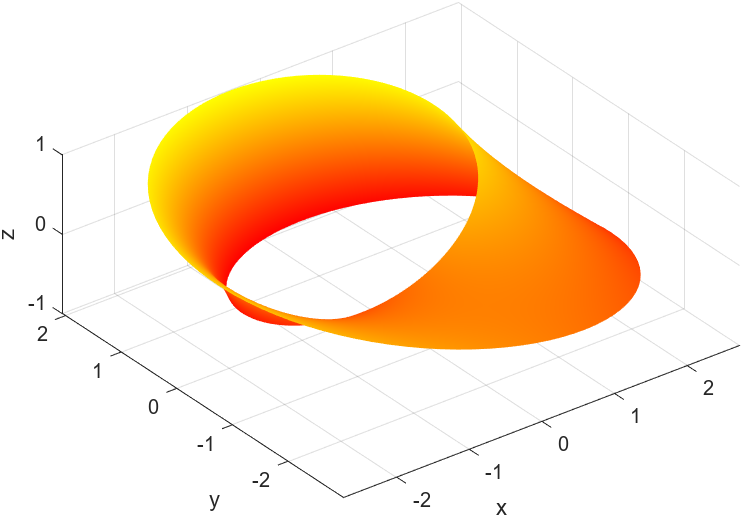
\includegraphics[width=\textwidth]{Capitoli/Capitolo6/Nastro di Moebius.png}
     \end{minipage}
     \begin{minipage}{0.55\textwidth}
        Una possibile parametrizzazione di tale superficie può essere
        \begin{equation*}
            r(u,v)= \begin{cases}
                \left(2-v \sin\left(\frac{u}{2}\right)\right) \sin(u)\\
                \left(2-v \sin\left(\frac{u}{2}\right)\right) \cos (u)\\
                v \cos\left(\frac{u}{2}\right)
            \end{cases}
        \end{equation*}
    con $u \in [0, 2\pi], v \in [-1,1]$
     \end{minipage}
 \end{figure}
 \begin{figure}[H]
     \centering
     \begin{minipage}{0.5\textwidth}
 In particolare, studiando i punti in cui $v$ sia nullo si ha che
 \begin{align*}
     & n=\frac{\partial r}{\partial u} \wedge \frac{\partial r}{\partial v}=(2\sin u, 2 \cos u, 0)\\
     &\lim_{u \to 0^+} n (u,0) = (0,-2,0)\\
     &\lim_{u \to 2\pi^-} n (u,0) = (0,2,0)
 \end{align*}
 e ciò non rispetta la definizione di superficie orientabile.
 \end{minipage}
 \begin{minipage}{0.3\textwidth}
     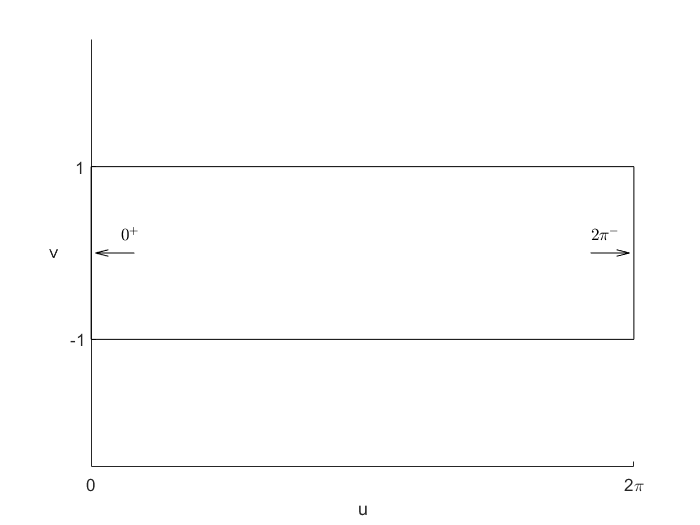
\includegraphics[width=\textwidth]{Capitoli/Capitolo6/Area per calcolo orientazione.png}
 \end{minipage}
 \end{figure}
 \end{example}
 \begin{example}
     Diversamente dal nastro di Möbius, si può osservare che i grafici di funzioni in due variabili $z=f(x,y)$ di classe $C^1$ sono superfici orientabili il cui sostegno è dato dal grafico $\mathcal{G}(f)$.
     Le equazioni parametriche della superficie sono:
     \begin{equation*}
         r(u,v)=\begin{cases}
             x= u\\
             y=v\\
             z=f(u,v)
         \end{cases}
     \end{equation*}
     Calcolando le derivate parziali ed il loro prodotto vettoriale si ha che
     \begin{equation*}
        \begin{aligned}
            &\frac{\partial r}{\partial u} = \left( 1, 0, \frac{\partial f}{\partial u}(u,v)\right)\\
            &\frac{\partial r}{\partial v} = \left( 0, 1, \frac{\partial f}{\partial v}(u,v)\right)\\
        \end{aligned}
            \qquad \Rightarrow \quad \nu(u,v)= \frac{\left(-\frac{\partial f}{\partial u}(u,v), -\frac{\partial f}{\partial v}(u,v), 1\right)}{\sqrt{1+ \left| \nabla f(u,v) \right|^2}}
     \end{equation*}
     Vale la pena notare che invertendo le variabili (ad esempio $x=v,\ y=u$) si ha un cambio di orientazione. Di conseguenza, l'orientazione dipende dalla parametrizzazione scelta.\\
     Inoltre, tramite il normale, è possibile distinguere tra "sopra" e  "sotto" o tra "dentro" e "fuori".
     \begin{figure}[H]
         \centering
         \begin{minipage}{0.4\textwidth}
         Si prenda ad esempio un paraboloide di equazione:
         \begin{align*}
             r(u,v)= \begin{cases}
                 x=u\\
                 y=v\\
                 z=u^2+v^2
             \end{cases}
         \end{align*}
        con $u \in [-1.5, +1.5],\ v \in [-1.5, +1.5]$.\\
        Calcolando, secondo le diverse convenzioni di segno, il versore normale è possibile visualizzare graficamente quanto asserito prima rispetto al "sopra" e "sotto".
     \end{minipage}
    \begin{minipage}{0.5\textwidth}
        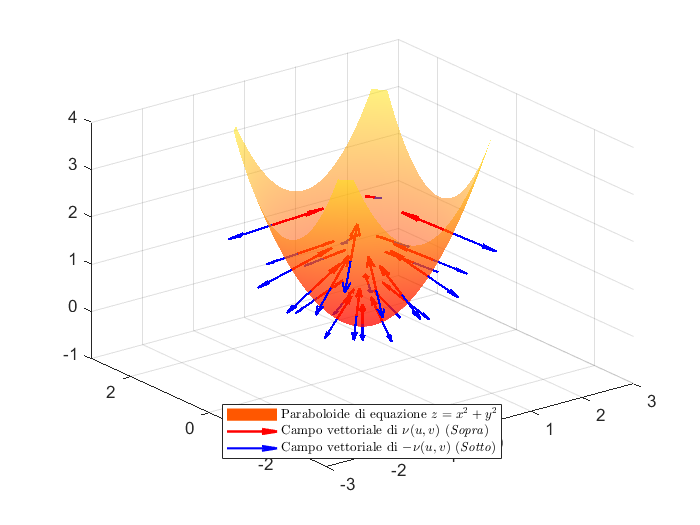
\includegraphics[width=\textwidth]{Capitoli/Capitolo6/Paraboloide.png}
    \end{minipage}
    \begin{minipage}{0.5\textwidth}
    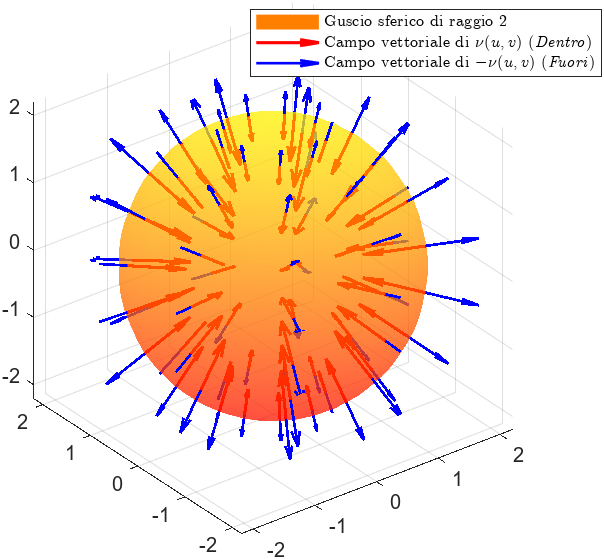
\includegraphics[width=\textwidth]{Capitoli/Capitolo6/Guscio sferico.png}
    \end{minipage}
    \begin{minipage}{0.4\textwidth}
    Discorso analogo, rispetto al "dentro" o "fuori" può essere fatto con un guscio sferico di raggio $R$ fissato. In figura $R=2$ con una superficie di parametrizzazione
    \begin{align*}
    r(u,v)=\begin{cases}
        x= R \sin u \cos v\\
        y= R \sin u \sin v\\
        z= R \cos u
    \end{cases}    
    \end{align*}
    con $u \in [0, 2\pi],\ v \in [0, \pi]$.
    \end{minipage}
    \end{figure}
 \end{example}
\section{Integrali superficiali}
\subsection{Area di una superficie}
Se, parlando di curve, era necessario definire il concetto di lunghezza, ora, trattando le superfici, occorre definire l'area.\\
È possibile costruire intuitivamente l'elemento infinitesimo di area $d \sigma$. Si considerino $D \subseteq \R^2$ dominio connesso limitato e una superficie regolare di parametrizzazione $r: D \to \R^3$ e si fissi un punto $(u_0, v_0) \in D$. Preso un rettangolo $R$ individuato dai punti $(u_0, v_0),\ (u+ \Delta u, v + \Delta v) \in \mathring{D}$ e detta $\Tilde{R}$  la sua immagine tramite $r$, si può approssimare l'area di $\Tilde{R}$ come l'area di un parallelogramma $\Pi$ avente un vertice in $r(u_0,v_0)$ e il lati paralleli e congruenti ai vettori $\tfrac{\partial r}{\partial u} (u_0,v_0) \Delta u$ e $\tfrac{\partial r}{\partial v}(u_0,v_0) \Delta v$. Dunque, l'area di $R$ è
\begin{equation}
\area(R)=|\Delta u||\Delta v|    
\end{equation}
 e quella di $\Pi$ è data da
 \begin{equation}
 \area(\Pi)= \left|\frac{\partial r}{\partial u} (u_0,v_0) \Delta u \wedge \frac{\partial r}{\partial v}(u_0,v_0) \Delta v \right|
 \end{equation}
 Di conseguenza, l'elemento infinitesimo di area $d \sigma$ in $r(u_0, v_0)$ è dato da
 \begin{equation}
     d\sigma= \left|\frac{\partial r}{\partial u} (u_0,v_0) \wedge \frac{\partial r}{\partial v}(u_0,v_0) \right|\, du\, dv
 \end{equation}
 \begin{definition} \label{Def: Area di una superficie}
     Siano $D \subseteq \R^2$ un dominio connesso limitato e $r: D \to \R^3$ una superficie regolare tale che $S=r(D)$. Allora si definisce l'\textbf{area} di $S$ come
     \begin{equation}
         \area(S)= \iint\limits_{S}{d\sigma} := \iint\limits_{D}{\left|\frac{\partial r}{\partial u} (u,v) \wedge \frac{\partial r}{\partial v}(u,v) \right|\, du\, dv}
     \end{equation}
 \end{definition}
 \begin{example}
     Si calcoli l'area di una sfera di raggio $R$ fissato.
     \begin{equation*}
         r(\vartheta, \varphi)=\begin{cases}
             x= R \sin \varphi \cos \vartheta\\
             y= R \cos \varphi \cos \vartheta\\
             z=R \cos \varphi
         \end{cases}
         \qquad \vartheta \in [0, 2\pi],\ \varphi \in [0, \pi]
     \end{equation*}
     Allora, l'elemento infinitesimo di area è $d\sigma= R^2 \sin \varphi\, d\varphi$ e 
     \begin{equation*}
         \area(r)= \iint\limits_{[0, \pi] \times [0, 2\pi]}{R^2 \sin \varphi}\, d\varphi= 2\pi R^2 \int\limits_{0}^{\pi}{\sin \varphi}\, d\varphi = 4\pi R^2
     \end{equation*}
 \end{example}
\subsection{Integrali superficiali di prima specie}
 \begin{definition} \label{Def: Integrale superficiale di prima specie}
     Sia $f: \Omega \subseteq \R^3 \to \R$ continua. Siano poi $D,\ r$ definiti come sopra e sia $S=r(D) \subseteq \Omega$. Allora si dice \textbf{integrale superficiale di prima specie}
     \begin{equation}
         \iint\limits_{S}{f}\, d\sigma = \iint\limits_{D}{f(r(u,v)) \left|\frac{\partial r}{\partial u} (u,v) \wedge \frac{\partial r}{\partial v}(u,v) \right|\, du\, dv}
     \end{equation}
 \end{definition}
 L'interpretazione grafica di tale integrale è quella del volume sotteso dal grafico $\mathcal{G}(f)$ valutato sulla superficie $S$.\\
 Un altro dettaglio che vale la pena evidenziare è che l'integrale superficiale definito è invariante per riparametrizzazioni equivalenti.
 \begin{oss}
     Bisogna tenere a mente che la parametrizzazione in coordinate cartesiane di una sfera di raggio $R$ centrate nell'origine è data dall'unione delle parametrizzazioni della semisfera inferiore e superiore, cioè, rispettivamente,
     \begin{equation}
         r_1(u,v)= \begin{cases}
             x= u\\
             y=v\\
             z=-\sqrt{R^2- u^2-v^2}
         \end{cases}
         \cup  \quad
         r_2(u,v)= \begin{cases}
             x=u\\
             y=v\\
             z=\sqrt{R^2- u^2-v^2}
         \end{cases}
     \end{equation}
     Inoltre, se la sfera ha un versore normale uscente, occorre che le due parametrizzazioni abbiano orientazione ad esso concorde.
 \end{oss}
 \begin{oss}
     Grazie all'integrale superficiale di prima specie è possibile esprimere le formule per il calcolo di massa $m$ e centro di massa $C$ di lamine curve. Sia $\varrho: S=r(D) \to +\infty$ la densità di una distribuzione di massa sulla superficie di sostegno $S$. Allora la massa totale è
     \begin{equation}
         m= \iint\limits_S{\varrho}\, d\sigma
     \end{equation}
     Il centro di massa $C$ invece ha coordinate
     \begin{equation}
         x_C= \frac{1}{m}\iint\limits_{S}{x \varrho}\, d\sigma, \quad y_C= \frac{1}{m}\iint\limits_{S}{y \varrho}\, d\sigma, \quad z_C= \frac{1}{m}\iint\limits_{S}{z \varrho}\, d\sigma
     \end{equation}
     Se poi $\varrho$ è costante, le formule per il calcolo del centro di massa offrono le coordinate del baricentro della lamina. 
 \end{oss}
 \subsection{Integrali superficiali di seconda specie}
 Prima di entrare nel vivo degli integrali superficiali di seconda specie, occorre trattare le \textit{superfici con bordo}. Tuttavia, poiché non si hanno a disposizione gli strumenti necessari per dare una definizione di bordo di una superficie, verrà data quella di \textit{bordo parametrico}, che è assolutamente sufficiente ai fini del calcolo di tali integrali.
 \begin{definition} \label{Bordo parametrico}
     Sia $r$ una superficie regolare con $r: D \to \R^3$ e $S=r(D)$ con $D$ definito come sopra. Allora si dice \textbf{bordo parametrico} di $S$ l'insieme
     \begin{equation}
         \partial_r S := r(\partial D)
     \end{equation}
 \end{definition}
 \begin{example}
     Si prenda un cilindro con base di raggio $R=2$ di parametrizzazione
     \begin{equation*}
         r(\varphi,t)=\begin{cases}
             x= R \cos \varphi\\
             y= R R \sin \varphi\\
             z=t
         \end{cases}
         \qquad \varphi \in [0, 2\pi],\ t \in [0, 2]
     \end{equation*}
     e si consideri la frontiera del suo dominio.
     La frontiera di $D$ è quella in figura. Si può osservare che
     \begin{align*}
         \partial_r S = r(0,t) = r(2\pi, t) \cup r(\varphi, 0) \cup r(\varphi, 2)
     \end{align*}
     \begin{figure}[H]
     \begin{minipage}{0.4\textwidth}
     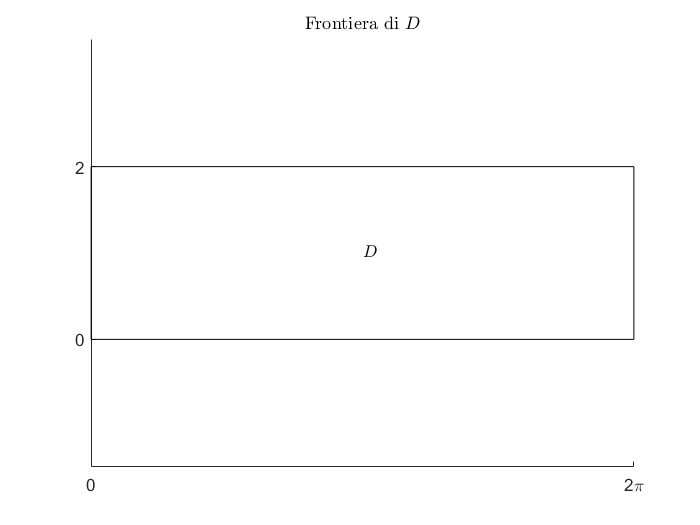
\includegraphics[width=\textwidth]{Capitoli/Capitolo6/Frontiera D.png}
     \end{minipage}
     \centering
     \begin{minipage}{0.5\textwidth}
     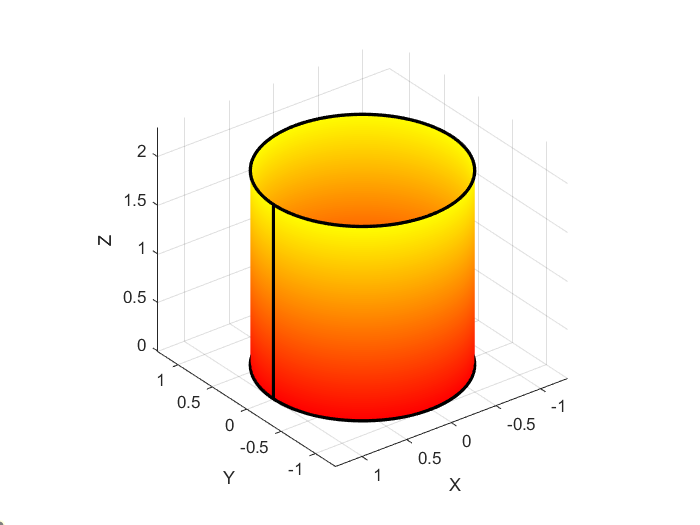
\includegraphics[width=\textwidth]{Capitoli/Capitolo6/Bordo parametrico cilindro.png}
     \end{minipage}
     \end{figure}
     In nero è mostrato il bordo parametrico.
 \end{example}
 \begin{definition} \label{Def: Superficie regolare con bordo}
     Sia $D \subseteq \R^2$ dominio regolare connesso tale che $D \subseteq A$ aperto. Allora si dice \textbf{superficie regolare con bordo} un'applicazione
     \begin{equation}
         r: A \to \R^3
     \end{equation}
     di classe $C^1(A)$ tale che $r$ sia semplice e che la sua Jacobiana $J_r(u,v)$ abbia rango $2$ per ogni $(u,v) \in D$.
 \end{definition}
 \begin{oss}
     Il rango massimo della Jacobiana garantisce che se il bordo di $D$ è unione di curve regolari a tratti $\gamma_i$, allora
     \begin{equation}
         r(\partial D)= \bigcup_{i=1}^N r(\gamma_i)
     \end{equation}
 \end{oss}
 \begin{oss}
     La parametrizzazione stessa della superficie offre un modo per orientare positivamente il bordo parametrico della stessa. In particolare si dice che $\partial_r S$ è \textbf{orientato positivamente} e lo si indica con $\ppartial_r S$ se
     \begin{equation}
         \ppartial_r S = \ppartial r( \ppartial D)
     \end{equation}
 \end{oss}
 \begin{definition} \label{Def: Versore normale positivo}
     Data una superficie regolare orientabile con bordo $\partial_r S$ si definisce il \textbf{versore normale positivo} come
     \begin{equation}
         \nu_+(u,v) = \frac{\frac{\partial r}{\partial u} (u,v) \wedge \frac{\partial r}{\partial v}(u,v)}{\left|\frac{\partial r}{\partial u}(u,v) \wedge \frac{\partial r}{\partial v}(u,v)\right|} \qquad \forall\ (u,v) \in D
     \end{equation}
 \end{definition}
 Fatte tali premesse è possibile definire l'integrale superficiale di seconda specie, o, in termini fisici, il flusso di un campo vettoriale $F$.
 \begin{definition} \label{Def: Integrale superficiale di seconda specie}
     Sia $F: S \to \R^3$ un campo vettoriale di classe $C^1$ e sia $S$ regolare. Allora si definisce il \textbf{flusso} di $F$ (o \textit{integrale superficiale di seconda specie}) attraverso $S$ nella direzione del normale $\nu$ come
     \begin{equation}
         \Phi_S(F) := \iint\limits_S{\langle F, \nu \rangle}\, ds
     \end{equation}
 \end{definition}
 \begin{oss}
     In realtà ai soli fini della definizione dell'integrale superficiale di seconda specie è sufficiente che $F$ sia di classe $C^0$.
 \end{oss}
  \begin{theorem}[Teorema di Stokes o del rotore] \label{Teo: Teorema di Stokes}
     Sia $r: D \to \R^3$ una superficie regolare orientabile con bordo $\partial_r S$. Sia $F \in C^1(A)$ un campo vettoriale con $A \subseteq \R^3$ aperto tale che $A \subseteq S=r(D)$. Allora,
     \begin{equation}
         \iint\limits_{S} {\langle \Rot(F), \nu_+ \rangle}\, d\sigma = \int\limits_{\ppartial S}{\langle F, T \rangle}\, d\sigma
     \end{equation}
 \end{theorem}
 \begin{oss}
     I versi dell'enunciato dipendono tutti dalla parametrizzazione scelta.
 \end{oss}
 Questo primo risultato permette di calcolare il flusso del rotore di un campo $F$ come la circuitazione del campo stesso, passando dal calcolo di un integrale superficiale di II specie ad uno curvilineo di II specie.
 \begin{theorem}[Teorema di Gauss o della divergenza] \label{Teo: Teorema della divergenza}
     Sia $\Omega \subseteq \R^3$ un dominio regolare e sia $F: \Omega \to \R^3$ un campo di classe $C^1$. Allora
     \begin{equation}
         \iint\limits_{\partial \Omega}{\langle F, \nu_e\rangle}\, d\sigma = \iiint\limits_{\Omega}{\Div(F)}\, dx\, dy\, dz
     \end{equation}
 \end{theorem}
 \begin{oss}
     Si noti che il versore normale $\nu_e$ ha un verso preciso, cioè quello uscente.
 \end{oss}
 L'utilità di questo secondo risultato è analoga a quella del primo. Così diviene possibile calcolare l'integrale della divergenza di un campo come il flusso dello stesso campo in direzione uscente, passando da un integrale superficiale di II specie a un integrale triplo.
 \begin{theorem}[Teorema della divergenza in $\R^2$]
     Sia $D \subseteq \R^2$ un dominio regolare $F=(F_1, F_2) \in C^1(D)$ un campo vettoriale. Allora 
     \begin{equation}
         \iint\limits_{D} {\Div(F)}\,dx\,dy = \int\limits_{\ppartial D}{\langle F, \nu_e \rangle}\,ds
     \end{equation}
 \end{theorem}
 \begin{proof}
     Applicando Gauss-Green \eqref{Teo: Formule di Gauss Green} si ha
     \begin{equation}
     \iint\limits_{D}{\Div(F)}\,dx\,dy=\iint\limits_{D}{\left(\frac{\partial F_1}{\partial x}+ \frac{\partial F_2}{\partial y}\right)}\,dx\,dy \overset{\text{G.G.}}{=} \int\limits_{\ppartial D}{F_1 dx - F_2 dy}
     \end{equation}
     dove $\ppartial D$ è il sostegno di una curva di parametrizzazione $\varphi(t)= (x(t), y(t)$. Allora il versore tangente è parallelo a $(x'(t), y'(t))$ e il normale, per orientazione positiva è dato da 
     \begin{equation}
         \nu_e(t)=\left(\frac{y'(t)}{\sqrt{x'(t)^2+y'(t)^2}}, -\frac{x'(t)}{\sqrt{x'(t)^2+y'(t)^2}} \right)
     \end{equation}
     Perciò
     \begin{equation}
         \begin{aligned}
             \int\limits_{\ppartial D}{\langle F, \nu_e \rangle}\,ds &= \int\limits_{a}^{b}{\left(\frac{F_1y'(t)}{\sqrt{x'(t)^2+y'(t)^2}} -\frac{F_2x'(t)}{\sqrt{x'(t)^2+y'(t)^2}} \right)\sqrt{(x'(t)^2+y'(t)^2}}\, dt\\
             &=\int\limits_{a}^{b}{(F_1 y'(t)- F_2 x'(t))}\, dt \overset{\text{G.G.}}{=} \int\limits_{\ppartial D}{F_1\,dy- F_2\,dx} = \iint\limits_{D}{\Div(F)}\,dx\,dy
         \end{aligned}
     \end{equation}
\end{proof}
\begin{corollary}[Integrazione per parti in $\R^3$]
    Sia $F= gV$ un campo vettoriale con $g:\Omega \subseteq \R^3\to \R$ e $V: \Omega \to \R^3$ tali che $g,\ V \in C^1(\Omega)$. Allora 
    \begin{equation}
    \iiint\limits_{\Omega}{g \Div(V)}= \iint\limits_{\partial \Omega}{g \langle V, \nu_e \rangle}\, d\sigma - \iiint\limits_{\Omega}{\langle \nabla g, V \rangle}\,dx\,dy\,dz
    \end{equation}
\end{corollary}
\begin{proof}
Poiché $\Div(F)= \langle \nabla, gV \rangle = \langle \nabla g, V \rangle + \langle g, \Div V \rangle$, allora, calcolare l'integrale triplo di $\Div(F)$ significa calcolare
    \begin{equation}
      \iiint\limits_\Omega{g \Div V}\,dx\,dy\,dz = \iiint\limits_{\Omega} {\Div(F)}\,dx\,dy\,dz - \iiint\limits_{\Omega} {\langle \nabla g, V \rangle}\,dx\,dy\,dz
    \end{equation}
    Dal teorema della divergenza si ha 
    \begin{equation}
    \iiint\limits_{\Omega}{g \Div(V)}= \iint\limits_{\partial \Omega}{g \langle V, \nu_e \rangle}\, d\sigma - \iiint\limits_{\Omega}{\langle \nabla g, V \rangle}\,dx\,dy\,dz
    \end{equation}
\end{proof}